Consider two identical homogeneous balls, A and B, with the same initial
temperatures. One of them is at rest on a horizontal plane, while the second one
hangs on a thread (Fig.~6). The same quantities of heat have been supplied to
both balls. Are the final temperatures of the balls the same or not? Justify
your answer. (All kinds of heat losses are negligible.)

\begin{center}
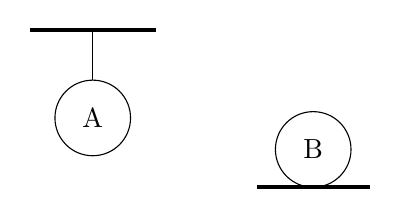
\begin{tikzpicture}[scale=0.8]
  \draw[line width=1.5pt] (-1,3) -- (1,3);
  \draw (0,3) -- (0,2.2);
  \draw (0,1.6) circle (0.6) node {A};
  \draw (3.5,1.1) circle (0.6) node {B};
  \draw[line width=1.5pt] (2.6,0.5) -- (4.4,0.5);
\end{tikzpicture}
\figcap{Fig.~6}
\end{center}
